% =========================================================================
% CHAPTER 2 — RESEARCH QUESTIONS & OBJECTIVES
% =========================================================================

\chapter{Research Questions \& Objectives}
\label{ch:rqs}

\noindent
{\rmfamily\itshape
\begin{tabular}[t]{@{}l@{\hspace{0.3cm}}p{12.5cm}@{}}
\textls[50]{\textbf{Addressed:}} &
\textls[50]{Key Research Questions · Issues to Address · Assumptions Requiring Validation · Project Objectives · Hypotheses}
\end{tabular}
}

% -------------------------------------------------------------------------
\section{Research Framework}
\label{sec:rq-framework}

Chapter~\ref{ch:introduction} identified a representational problem: complex climate tipping systems stay cognitively out of reach for non-specialists even when the data are open and legible. This chapter formalises the programme that addresses it. The programme follows the three-phase arc of \emph{detect, translate and evaluate}, adapted from design-based research in the learning sciences, where designing a solution is itself treated as research \citep{andersonshattuck2012, barab2004}. The phases are linked: what is detected sets what can be translated, and what is translated becomes what is evaluated. A single central research question connects them, and three sub-questions --- one per phase --- investigate it through different kinds of evidence.

The three phases do not weigh equally.\footnote{The \emph{detect} phase is analytical and largely complete; the \emph{evaluate} phase is exploratory, offering an initial assessment rather than definitive validation.} The centre of gravity is the bridge between the first two: translating machine-learning-derived structure into representations built to improve understanding. That bridge is the original methodological contribution; the evaluation asks whether it shows promise, within the limits of a small exploratory study.

% -------------------------------------------------------------------------
\section{Research Questions}
\label{sec:rqs}

The central question guides the thesis as a whole, and is deliberately evaluative rather than merely design-oriented:

\begin{quote}
\textbf{RQ.} \emph{To what extent do machine-learning-driven experiential visualisations improve the cognitive understanding of complex climate tipping systems among non-specialist audiences, compared with conventional static visualisations?}
\end{quote}

Every element is a choice. The construction \emph{to what extent\ldots compared with} sets a comparative frame: the aim is not to build a visualisation but to test whether it supports understanding better than a conventional one. Therefore, design is the means; evaluation is the end. \emph{Non-specialist audiences} names participants characterised by background, not an undefined public; \emph{complex climate tipping systems} names the class of processes for which the AMOC is the case study. The thesis does not ask whether machine learning can predict or detect an AMOC tipping point --- a question still debated in climate science \citep{benyami2024, ditlevsen2023} --- but whether the latent structure it recovers can be translated into representations that help non-specialists understand an otherwise invisible system.

Three sub-questions follow the three phases:

\begin{quote}
\textbf{RQ1} (analytical). \emph{What latent structural patterns and dynamical signatures of AMOC variability can machine learning recover from the RAPID record and the Copernicus reanalysis ensemble, and how faithfully do they preserve the underlying dynamics relative to classical statistical approaches?}
\end{quote}

RQ1 is descriptive and exploratory. It commits the thesis not to a new oceanographic result but to an honest account of what the data hold. The load-bearing word is \emph{faithfully}: the contribution is not that a method was applied, but that the low-dimensional representation is shown to preserve the system's structure, and so earns the right to serve as the substrate for what follows.

\begin{quote}
\textbf{RQ2} (design-based). \emph{How can the latent structures from RQ1 be translated into interactive and experiential representations that communicate the AMOC's dynamics, invisibility and tipping-point risk, grounded in embodied cognition and information visualisation?}
\end{quote}

RQ2 is generative: it has no single correct answer, but a class of well-justified ones to construct and defend. It produces the representations that RQ3 evaluates --- not the endpoint, but the object of study.

\begin{quote}
\textbf{RQ3} (empirical). \emph{To what extent do dynamic and experiential representations of AMOC dynamics, compared with a conventional static one, support how non-specialist audiences develop and express their understanding of complex system behaviour?}
\end{quote}

RQ3 is comparative but exploratory. It does not measure effectiveness at population scale; it observes how participants describe and organise their understanding under one representation or the other. Its wording mirrors the central question by design --- \emph{to what extent}, \emph{compared with} --- because it is a focused instance of the same enquiry, resting on qualitative depth rather than statistical generalisation. No sub-question answers the central one alone: RQ1 finds the structure, RQ2 builds the representation, RQ3 tests it against the baseline.

% -------------------------------------------------------------------------
\section{Objectives}
\label{sec:objectives}

Each sub-question becomes a set of objectives with defined outputs, tied in the alignment matrix (Table~\ref{tab:alignment}) to the chapter that delivers them and the claim they advance.

The analytical objectives structure Chapter~\ref{ch:data_pipeline}. They recover the latent vertical structure of the AMOC through principal component analysis (\textbf{O1.1}), test whether that structure is genuinely low-dimensional by comparing it against a non-linear autoencoder at matched dimensionality (\textbf{O1.2}), characterise the record's anomalies and test for early-warning signals under a corrected significance test (\textbf{O1.3}), and specify --- but defer to future work --- a probabilistic forecasting layer (\textbf{O1.4}).

The design objectives structure Chapter~\ref{ch:translate}. They define the three representational conditions on shared information (\textbf{O2.1}), develop the transferable design grammar that maps machine-learning features onto perceptual channels (\textbf{O2.2}), and encode the boundary between observation and projection as a felt perceptual quality rather than a numerical annotation (\textbf{O2.3}).

The empirical objectives structure Chapters~\ref{ch:userstudy} and~\ref{ch:results}. They build the mixed-methods instrument (\textbf{O3.1}), run the two-group study (\textbf{O3.2}), and assess whether the machine-learning-derived perceptual encodings are read by participants as intended (\textbf{O3.3}).

% -------------------------------------------------------------------------
\section{Hypotheses and Design Propositions}
\label{sec:hypotheses}

The sub-questions differ in kind, so the claims are framed accordingly: RQ1 admits directional \emph{hypotheses}; RQ2 advances \emph{design propositions} assessed against design criteria; RQ3 states exploratory \emph{expectations}. Treating these as equivalent would misrepresent the evidence each can bear \citep{cronbach1975, mckenney2018}. Two umbrella hypotheses frame the whole: that conventional static representations are insufficient for non-specialists, presenting complexity as information to read rather than a process to grasp (\textbf{H-A}); and that machine-learning-derived representations, made dynamic and experiential, can change how non-specialists understand system behaviour by rendering its structure perceptible, not by replacing analysis (\textbf{H-B}).

The analytical hypotheses are directional and reported in Chapter~\ref{ch:data_pipeline}. \textbf{H1}: a few linear modes explain most of the variance in the AMOC vertical profiles \citep{buckley2016, hannachi2007}. \textbf{H2}: a non-linear autoencoder does not materially outperform PCA at equal dimensionality, so interpretable linear coordinates lose little \citep{baldi1989}. \textbf{H3}: once the effective sample size is corrected for autocorrelation in overlapping windows, classical Early Warning Signals show no significant trend across the RAPID record.\footnote{H3 is deliberately framed around a null result. Showing that an apparent signal disappears once statistical dependence is handled correctly is not a failure but a demonstration of methodological robustness \citep{dakos2012, scheffer2009}.}

The design propositions are realised in Chapter~\ref{ch:translate}. \textbf{DP2.1}: machine-learning features --- latent position, anomaly score, ensemble uncertainty --- can be mapped onto perceptual dimensions such as colour, motion, density and sound, consistent with pre-attentive processing and embodied cognition \citep{lakoff1999, ware2021}. \textbf{DP2.2}: the boundary between observation and projection can be encoded as a felt perceptual transition rather than a numerical annotation.

The empirical expectations guide the qualitative analysis. \textbf{E3.1}: the experimental group will describe AMOC behaviour --- its dynamics, non-linearity, invisibility --- in qualitatively different ways from the control group, whether or not this matches measurable gains in the comprehension probe. \textbf{E3.2}: the perceptual encoding of uncertainty will produce interpretations the final survey and analysis can surface, whether or not they match the intended reading. Neither presumes a direction or magnitude of effect.

% =========================================================================
% figures/rq_tree.tex — Research-questions tree (loads pre-compiled PDF)
% Requires \usepackage{graphicx} in the preamble.
% Insert in the chapter with: % =========================================================================
% figures/rq_tree.tex — Research-questions tree (loads pre-compiled PDF)
% Requires \usepackage{graphicx} in the preamble.
% Insert in the chapter with: % =========================================================================
% figures/rq_tree.tex — Research-questions tree (loads pre-compiled PDF)
% Requires \usepackage{graphicx} in the preamble.
% Insert in the chapter with: \input{figures/rq_tree.tex}
% =========================================================================

\begin{figure}[!ht]
    \centering
    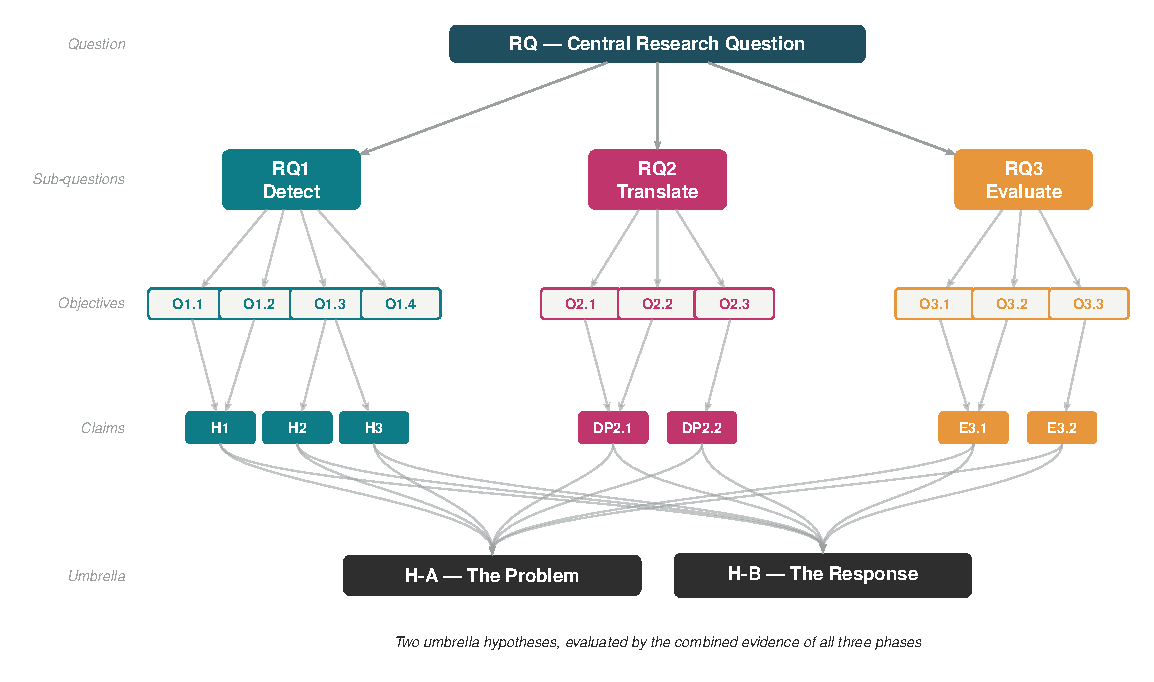
\includegraphics[width=\textwidth]{figures/research_questions/rq_tree_preview.pdf}
    \caption[Structure of the research questions, objectives, claims and umbrella hypotheses.]{\textbf{The
    architecture of the research programme.} The central research question branches into three
    sub-questions along the detect--translate--evaluate arc. Each sub-question generates its objectives
    (O1.1--O1.4, O2.1--O2.3, O3.1--O3.3), which give rise to the claims appropriate to their epistemic
    character: directional hypotheses (H1--H3), design propositions (DP2.1--DP2.2) and empirical
    expectations (E3.1--E3.2). All three claim groups converge on the two umbrella hypotheses, H-A (the
    problem) and H-B (the response), assessed not by any single instrument but by the combined evidence
    of the whole programme.}
    \label{fig:rq-tree}
\end{figure}
% =========================================================================

\begin{figure}[!ht]
    \centering
    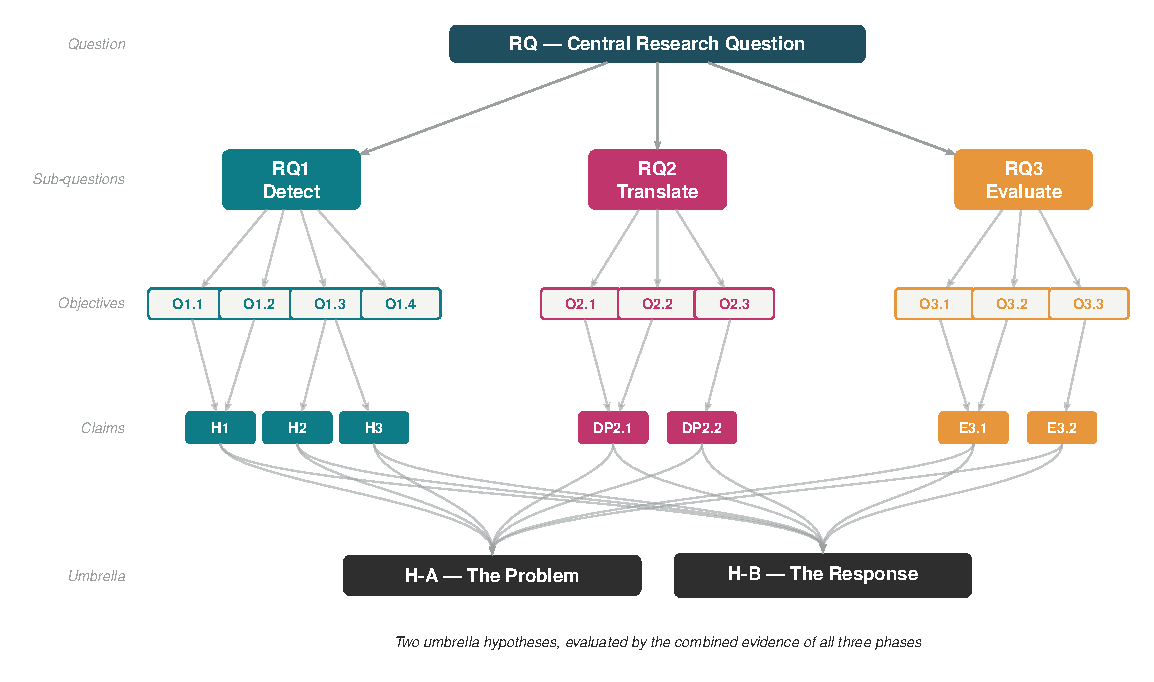
\includegraphics[width=\textwidth]{figures/research_questions/rq_tree_preview.pdf}
    \caption[Structure of the research questions, objectives, claims and umbrella hypotheses.]{\textbf{The
    architecture of the research programme.} The central research question branches into three
    sub-questions along the detect--translate--evaluate arc. Each sub-question generates its objectives
    (O1.1--O1.4, O2.1--O2.3, O3.1--O3.3), which give rise to the claims appropriate to their epistemic
    character: directional hypotheses (H1--H3), design propositions (DP2.1--DP2.2) and empirical
    expectations (E3.1--E3.2). All three claim groups converge on the two umbrella hypotheses, H-A (the
    problem) and H-B (the response), assessed not by any single instrument but by the combined evidence
    of the whole programme.}
    \label{fig:rq-tree}
\end{figure}
% =========================================================================

\begin{figure}[!ht]
    \centering
    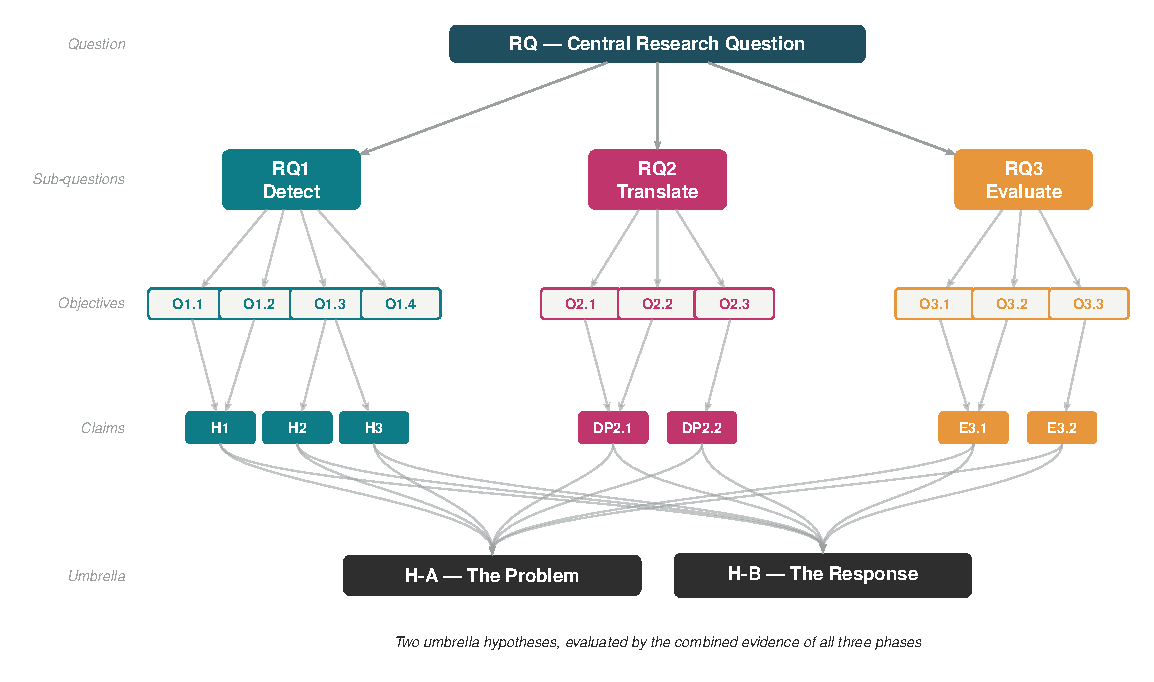
\includegraphics[width=\textwidth]{figures/research_questions/rq_tree_preview.pdf}
    \caption[Structure of the research questions, objectives, claims and umbrella hypotheses.]{\textbf{The
    architecture of the research programme.} The central research question branches into three
    sub-questions along the detect--translate--evaluate arc. Each sub-question generates its objectives
    (O1.1--O1.4, O2.1--O2.3, O3.1--O3.3), which give rise to the claims appropriate to their epistemic
    character: directional hypotheses (H1--H3), design propositions (DP2.1--DP2.2) and empirical
    expectations (E3.1--E3.2). All three claim groups converge on the two umbrella hypotheses, H-A (the
    problem) and H-B (the response), assessed not by any single instrument but by the combined evidence
    of the whole programme.}
    \label{fig:rq-tree}
\end{figure}

% -------------------------------------------------------------------------
\section{Alignment Matrix}
\label{sec:alignment-matrix}

The alignment matrix (Table~\ref{tab:alignment}) sets the three sub-questions against the operational structure of the thesis. Read down each column, it shows three coherent programmes --- analytical, design, empirical; read across each row, it shows how each phase feeds the next. It works as a promissory contract: for every commitment made here, a locatable delivery in a later chapter.

% -------------------------------------------------------------------------
\section{Feasibility and Scope Discipline}
\label{sec:rq-feasibility}

Feasibility rests on infrastructure, time and scope control. Most infrastructure is in place: the analytical phase is substantially complete, with the RAPID record and Copernicus ensemble processed and reported in Chapter~\ref{ch:data_pipeline}, so O1.1--O1.3 are implemented and O1.4 is specification only. The empirical phase requires a modest setup---a 20-minute survey administered to a target sample of approximately 20--30 participants, randomly divided into two groups: a static, conventional condition serving as the control group, and an experiential condition featuring interactive and machine-learning-powered visualisations. This sample size is appropriate for an exploratory first-stage study, aimed at identifying initial patterns in participants' cognitive understanding, rather than supporting statistically powered population-level inference \citep{braunclarke2006, smithmcgannon2018}. The design phase is the main remaining technical work, developed across Chapters~\ref{ch:methodology} and~\ref{ch:translate}.

Time is the main constraint, with completion planned for early September 2026. Theoretical and analytical writing comes first, so the riskiest part --- building the experiential condition --- happens once the surrounding text is settled. Keeping scope narrow is therefore a methodological choice: forecasting is left aside to keep the thesis on representation rather than prediction \citep{sonnewald2021}; the prototype stays a research artefact; and the study remains mainlyexploratory and qualitative. Two fallback plans keep the thesis coherent: if the study runs late, the analytical and design chapters stand alone; and if the experiential build fails technically, the design grammar still counts as a contribution (O2.2), defensible through the simpler conditions. The thesis is ambitious but focused --- each objective matched to the time available, each claim to the evidence it can carry.

\begin{table}[!ht]
    \centering
    \small
    \setlength{\tabcolsep}{5pt}
    \renewcommand{\arraystretch}{1.25}
    \caption{Alignment between the three sub-questions and the operational structure of the thesis, including how each is validated and against what criterion.}
    \label{tab:alignment}
    \begin{tabular}{
        @{}
        >{\RaggedRight\arraybackslash}p{2.7cm}
        >{\RaggedRight\arraybackslash}p{3.7cm}
        >{\RaggedRight\arraybackslash}p{3.7cm}
        >{\RaggedRight\arraybackslash}p{3.7cm}
        @{}
    }
        \toprule
        & \textbf{RQ1 --- Detect}
        & \textbf{RQ2 --- Translate}
        & \textbf{RQ3 --- Evaluate} \\
        \midrule
        \makecell[l]{\textbf{Epistemic}\\\textbf{character}}
            & Analytical, comparative, exploratory
            & Design-based, generative
            & Empirical, qualitative, comparative \\[0.5em]

        \textbf{Chapters}
            & Ch.~\ref{ch:background}, Ch.~\ref{ch:data_pipeline}
            & Ch.~\ref{ch:methodology}, Ch.~\ref{ch:translate}
            & Ch.~\ref{ch:methodology}, Ch.~\ref{ch:userstudy}, Ch.~\ref{ch:results} \\[0.5em]

        \textbf{Objectives}
            & O1.1--O1.4
            & O2.1--O2.3
            & O3.1--O3.3 \\[0.5em]

        \textbf{Claims}
            & H1, H2, H3
            & DP2.1, DP2.2
            & E3.1, E3.2 \\[0.5em]

        \textbf{Material}
            & RAPID observations, Copernicus reanalysis ensemble
            & Latent structures recovered in RQ1
            & Conditions produced in RQ2; non-specialist participants \\[0.5em]

        \textbf{Validation method}
            & Comparative model analysis: PCA vs.\ autoencoder at matched dimensionality; EWS with pseudo-replication correction; IsolationForest
            & Design-science construction against the grammar (Table~\ref{tab:design-grammar}); shared-provenance audit of informational equivalence
            & Between-subjects study, approximately 20--30 non-specialist participants, randomly assigned to static control and interactive, ML-powered experiential conditions; survey-based evaluation and exploratory analysis \\[0.5em]

        \textbf{Success criterion}
            & Latent gap $\leq$ reconstruction error; null trend correctly identified, not forced
            & Every on-screen value traceable to the bundle; conditions equivalent by construction of provenance
            & Experimental group articulates structure the control group does not, in spontaneous description \\[0.5em]

        \textbf{Output}
            & Latent-structure analysis; EWS null result; anomaly characterisation
            & Three representational conditions; documented design grammar
            & Anonymised responses; deductive codebook analysis against a pre-specified grid; descriptive two-group comparison \\[0.5em]

        \textbf{SDG anchoring}
            & 13 (Climate Action), 14 (Life Below Water)
            & 4 (Quality Education), 13
            & 4, 13 \\[0.5em]

        \textbf{Scope discipline}
            & LSTM forecasting deferred to future work
            & Research prototype, not production artefact
            & Exploratory two-group comparison; qualitative-primary, not statistically powered \\
        \bottomrule
    \end{tabular}
\end{table}